\chapter{ANNOTATION SYSTEM FOR MEDICAL DATA WITH SMART ASSISTANCE}
\label{sec:ANNOTATION SYSTEM FOR MEDICAL DATA WITH SMART ASSISTANCE}
\begin{ChapAbstract}
Chapter 4 details the design, implementation, and evaluation of an integrated AI assistant for smart navigation. This chapter presents a comprehensive system architecture that unifies multiple components: a data generation module, a cloud-based Firebase database with a hierarchical data structure, and an AI assistant powered by a state-of-the-art large language model (LLM) for natural language processing. It further explains the development of AI navigation capabilities using the Vuforia Engine and Creator App to enable real-time augmented reality experiences. The chapter also describes the user interface design—including an interactive home screen, AR navigation overlays, and a dedicated Q\&A metadata generation application—ensuring a seamless and intuitive user experience. A detailed demo plan is provided to illustrate the system's performance in diverse indoor environments.
\end{ChapAbstract}

\section{System Architecture}
This section presents an overview of the platform's system architecture, which is designed to be modular, scalable, and responsive for data annotation workflows. Figure~\ref{fig:system-architecture} illustrates the interconnected components that form the platform's ecosystem, comprising a client-side web application, a cloud-hosted serverless backend, and integrations with specialized external services.

\begin{figure}[ht]
\centering
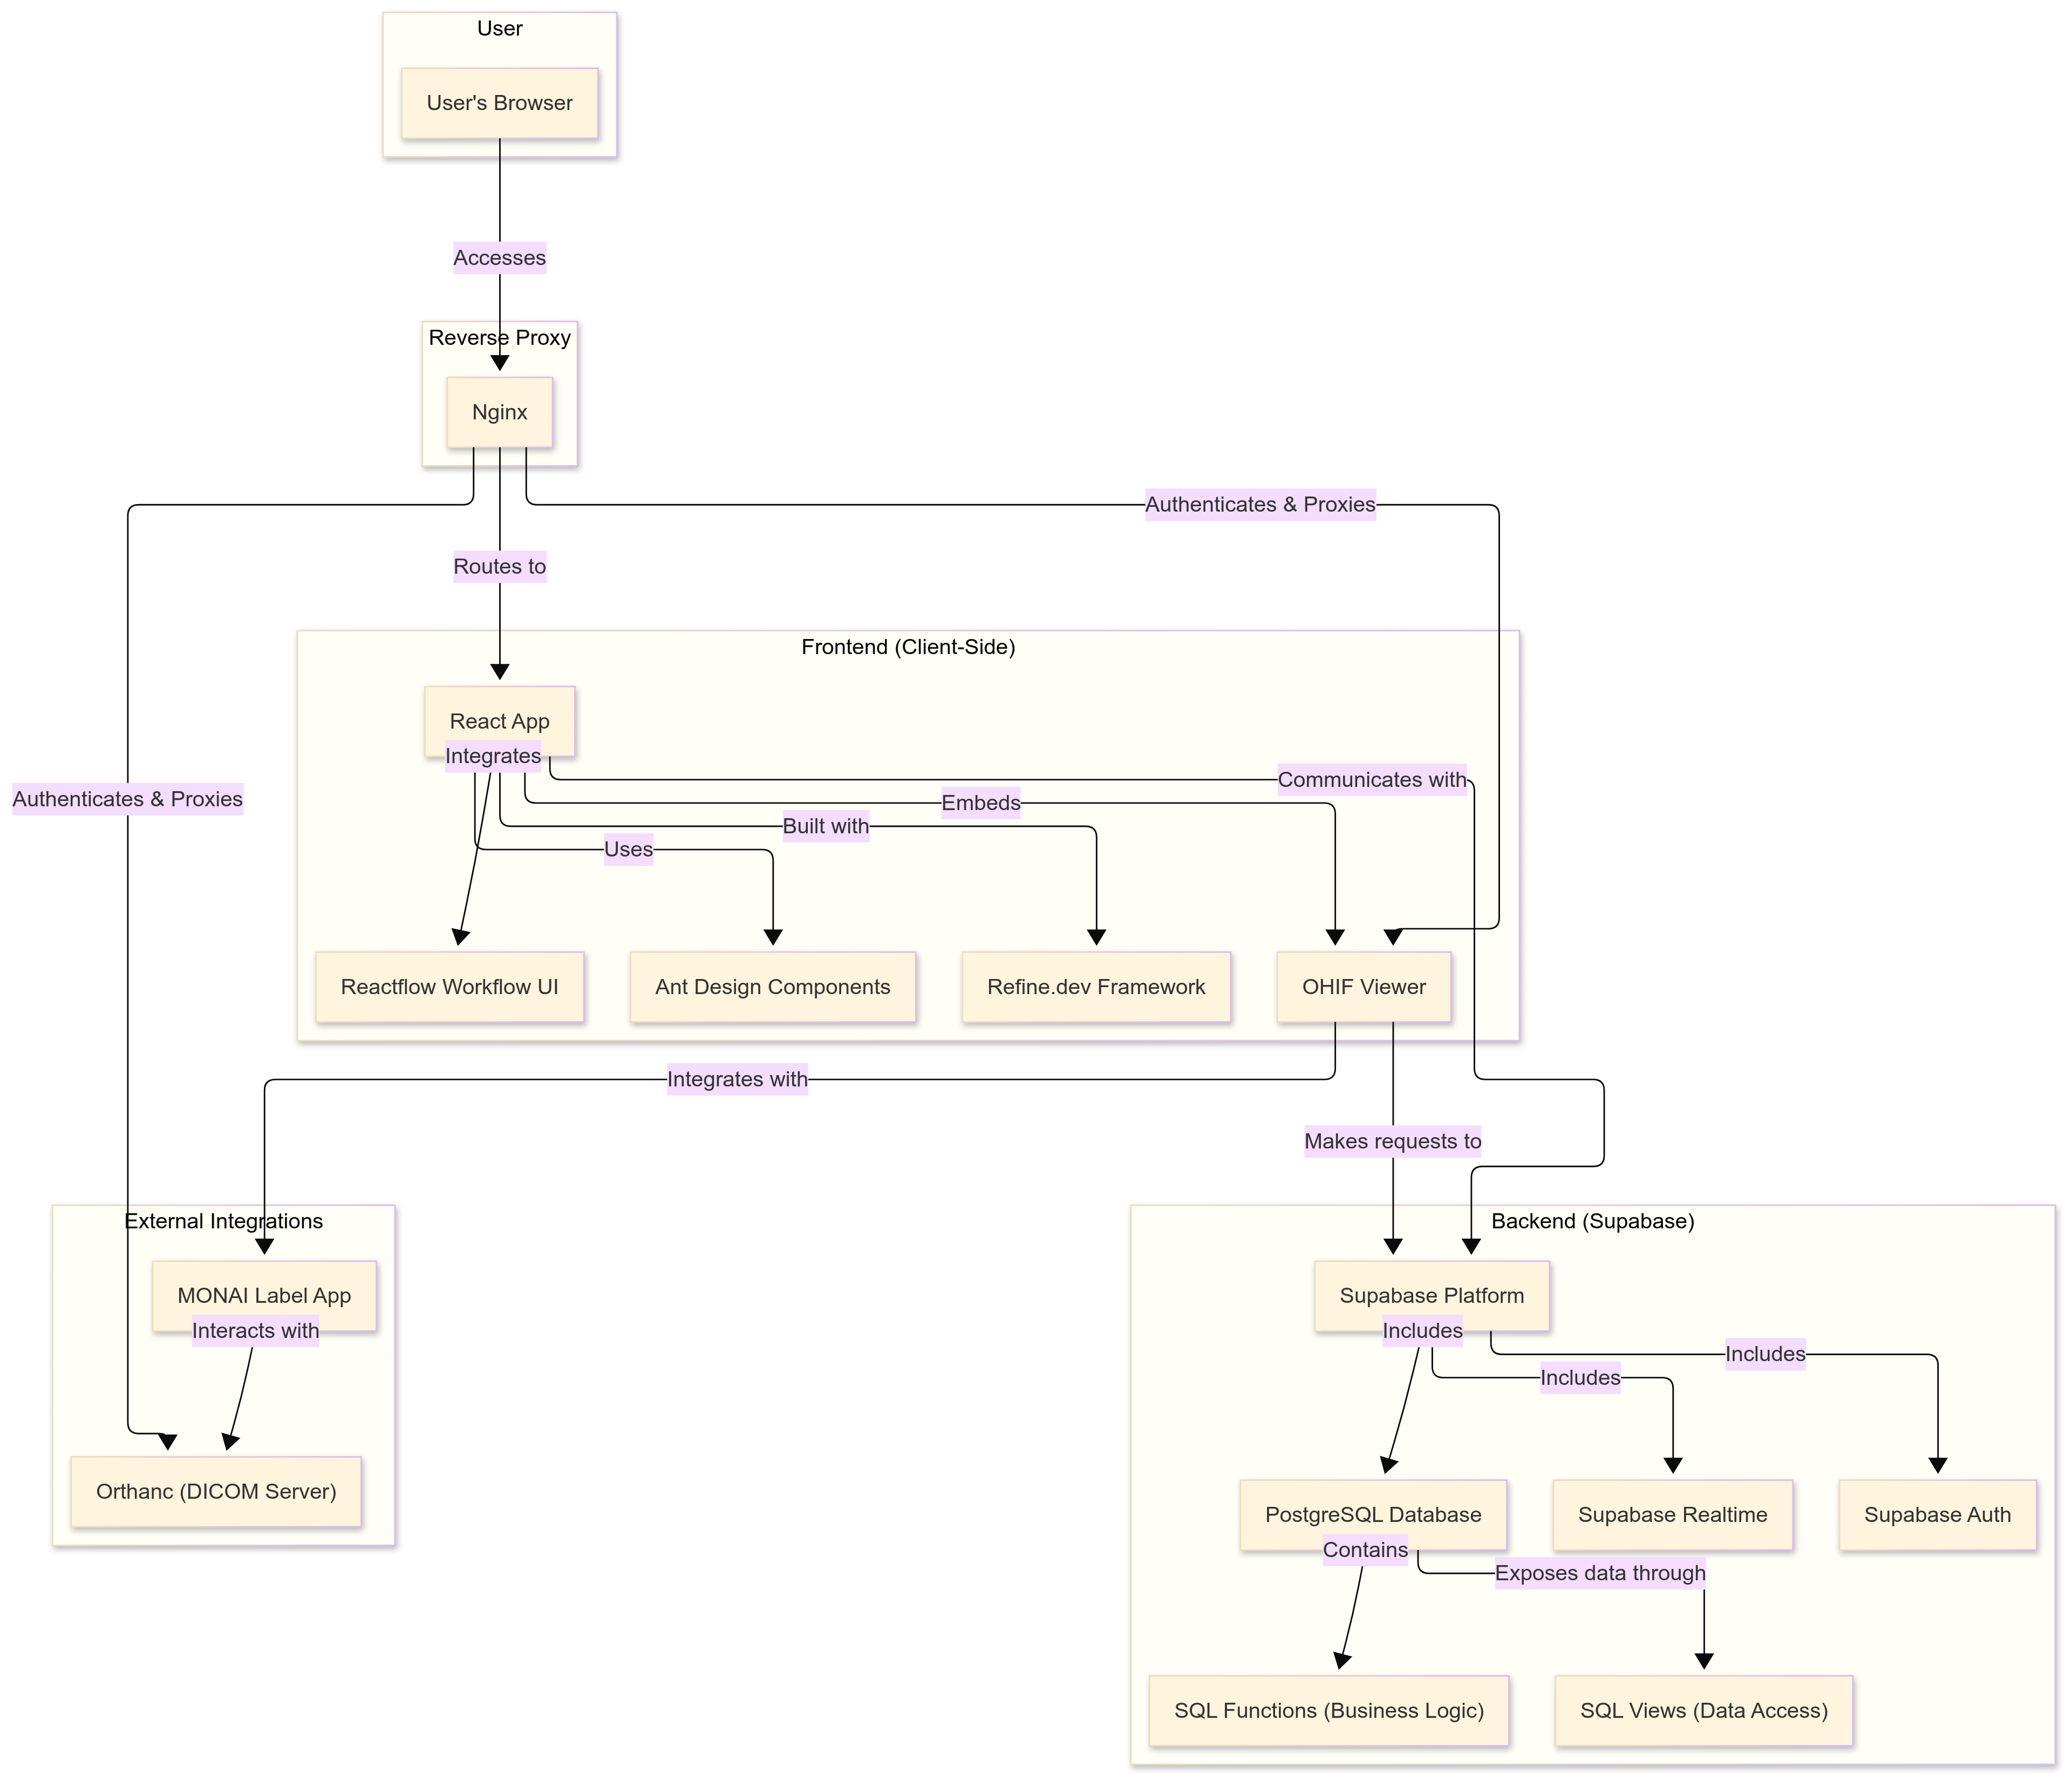
\includegraphics[width=0.9\textwidth]{content/resources/architecture.png} % Placeholder for diagram
\caption{Overall System Architecture.}
\label{fig:system-architecture}
\end{figure}

\subsection{Client-Side Application}
The client-side application provides the user interface for interacting with the platform. It runs within a standard web browser and is responsible for data presentation, user input, and real-time visualization of workflows and annotations.

\subsubsection{Web Browser Interface}
Users access the platform through a modern web browser. A dedicated Nginx reverse proxy manages traffic routing, serving the frontend assets and securely proxying specific requests to external services where necessary.

\subsubsection{Frontend Technologies}
The user interface is built as a React application, utilizing the \texttt{Refine.dev} framework to streamline development of CRUD operations and application logic. Visual consistency is provided by \texttt{Ant Design} components. For workflow design, the platform integrates \texttt{XYFlow} to enable interactive graphical editing of workflow graphs. Additionally, the \texttt{OHIF Viewer} is embedded for specialized medical imaging annotation and viewing functionalities.

\subsection{Backend Services (Supabase)}
The backend operates on a serverless architecture, leveraging Supabase to provide core database, authentication, and real-time capabilities.

\subsubsection{Supabase Ecosystem}
The entire backend resides within the Supabase platform, which provides a comprehensive suite of cloud-hosted services. This includes a robust \texttt{PostgreSQL Database} for all data storage, \texttt{Supabase Auth} for user authentication and authorization, and \texttt{Supabase Realtime} for instant data synchronization to connected clients.

\subsubsection{Data Storage and Logic}
All persistent data and core business logic are managed within the PostgreSQL database. This includes structured data for projects, tasks, and users, along with JSONB fields for flexible workflow stage configurations. Complex operations and state transitions are encapsulated within \texttt{SQL Functions}, which serve as the primary executable logic, while \texttt{SQL Views} provide abstracted and secure data access layers for the frontend.

\subsection{External Integrations}
The platform extends its capabilities through seamless integration with specialized external systems, particularly relevant for advanced medical imaging and AI-assisted annotation.

\subsubsection{Specialized Tools}
For AI-assisted medical image labeling, the platform integrates with the \texttt{MONAI Label App}, a server-side framework that offers machine learning model inference. Additionally, \texttt{Orthanc}, a lightweight DICOM server, functions as a primary source for medical image data, providing seamless access to studies for annotation tasks.
Generated latex
\section{System Requirements}

This section outlines the hardware and software prerequisites for deploying and utilizing the data annotation platform. The system is designed as a web-based application, with a distinct client-side interface and a cloud-hosted backend.

\subsection{Client-Side Requirements}
This section details the prerequisites for end-users interacting with the platform's web-based frontend.

\subsubsection{Software Requirements}
\begin{itemize}
    \item \textbf{Web Browser:} A modern web browser (e.g., Google Chrome, Mozilla Firefox, Microsoft Edge, Apple Safari) is required. The browser must support contemporary web standards, including JavaScript and CSS, for proper rendering and interactive functionality of the React-based frontend developed with Refine.dev and Ant Design.
    \item \textbf{Internet Connectivity:} A stable and reliable internet connection is essential for users to access the platform's cloud-hosted backend, retrieve project data, submit annotations, and receive real-time updates through Supabase's real-time capabilities.
\end{itemize}

\subsubsection{Hardware Recommendations}
\begin{itemize}
    \item \textbf{Device Type:} A desktop or laptop computer is recommended for optimal user experience. This allows for a larger screen area and precise input methods, which are beneficial for detailed annotation tasks and complex workflow graph design.
    \item \textbf{Processing Power \& Memory:} Devices should possess sufficient computing resources, typically 8GB of RAM or more and a modern multi-core CPU, to ensure smooth operation of demanding web applications, efficient rendering of intricate user interface components, and responsive interaction with large datasets that may be displayed in the browser.
    \item \textbf{Display Resolution:} A minimum screen resolution of 1920x1080 pixels is advisable. This ensures that all components of the user interface, particularly the interactive workflow editor and the integrated annotation tools, are displayed comprehensively without excessive scrolling or scaling.
\end{itemize}

\subsection{Server-Side Requirements}
This section outlines the infrastructure and software prerequisites for hosting and operating the platform's backend services and database.

\subsubsection{Supabase Backend Infrastructure}
The platform's backend is fundamentally architected around the \textbf{Supabase} ecosystem. This choice simplifies deployment and management by providing an integrated suite of services:
\begin{itemize}
    \item \textbf{PostgreSQL Database:} As the core data store, a PostgreSQL instance (version 12 or later recommended) is required. Supabase natively provides this, offering robust support for concurrent connections, efficient handling of JSONB data types for flexible configurations, and the execution of custom PL/pgSQL functions that encapsulate all backend business logic and workflow automation. Adequate and scalable disk space within the PostgreSQL environment is necessary to accommodate project data, tasks, annotations, and the comprehensive audit trail.
    \item \textbf{Integrated Services:} Supabase natively includes \textbf{Supabase Auth} for robust user authentication and authorization, and \textbf{Supabase Realtime} for real-time data synchronization.
    \item \textbf{System Automation:} The platform's automated workflow orchestration relies heavily on scheduled PostgreSQL functions acting as cron jobs. Supabase's architecture inherently supports the reliable execution of these functions at regular intervals, which is critical for triggering automated tasks assigned to virtual users and ensuring continuous workflow progression.
\end{itemize}
As an open-source platform, Supabase can be deployed as a managed cloud service or self-hosted, including via Docker container images, offering flexibility in infrastructure provisioning.

\subsubsection{External System Integrations}
The platform's comprehensive functionality is significantly enhanced through its ability to integrate with specialized external systems.
\begin{itemize}
    \item \textbf{Medical Imaging Archives (e.g., Orthanc):} For projects involving medical imaging data, network connectivity and appropriate API access permissions are required to integrate with external PACS (Picture Archiving and Communication System) or VNA (Vendor Neutral Archive) systems, such as Orthanc, for importing data items.
    \item \textbf{Annotation Toolkits (e.g., OHIF Viewer, MONAI):} While these are typically client-side components or frameworks leveraged for specific annotation tasks, the backend may require configured endpoints or data exchange protocols to seamlessly interact with instances of OHIF Viewer or MONAI, whether they are hosted externally or bundled within the client environment.
    \item \textbf{Machine Learning Models:} For advanced features like Model-Assisted Labeling (MITL), the backend requires stable network access to external machine learning model API endpoints. This includes consistent connectivity and valid API keys or authentication credentials to securely invoke these services for inference or prediction.
\end{itemize}

\subsubsection{Security \& Permissions}
\begin{itemize}
    \item \textbf{API Keys and Credentials Management:} Secure storage and management of API keys, access tokens, and other credentials for Supabase, external machine learning models, and any integrated third-party data sources (e.g., Orthanc) are paramount to maintaining system security.
    \item \textbf{Network Configuration:} Appropriate firewall rules and network security policies must be implemented on the server infrastructure to allow only necessary inbound and outbound connections for the backend services and external integrations, while strictly adhering to a strong security posture.
\end{itemize}

Here's the updated LaTeX code, with the figures integrated and captions updated. I've used X.Y as placeholders for chapter and figure numbers, as requested, and made sure the image paths are correct.

Generated latex
\section{Platform Features}
This section provides a comprehensive overview of the data annotation platform's features, highlighting its core functionalities, architectural design principles, and collaborative capabilities. The design emphasizes modularity, scalability, and an intuitive user experience, while leveraging a robust backend for automated processes.

\subsection{Authorization and Access Control}
The platform incorporates a sophisticated authorization system designed for granular control over resources and actions, ensuring data security and user privacy.

\subsubsection{Attribute-Based Access Control (ABAC)}
Instead of rigid, static roles, the system employs Attribute-Based Access Control (ABAC). Permissions are dynamically evaluated based on various attributes, including those of the user (e.g., role within a project), the resource (e.g., project, task, assignment), and the specific action being attempted (e.g., `create`, `delete`, `comment`). This enables highly flexible and fine-grained security policies.

\subsubsection{Contextual and Secure Authentication}
Access decisions are inherently contextual, with user permissions determined by their specific role within a given project. User authentication is securely managed through Supabase Auth, and user profiles store additional attributes (e.g., full name, avatar) that can further inform access control policies.

\begin{figure}[h!]
    \centering
    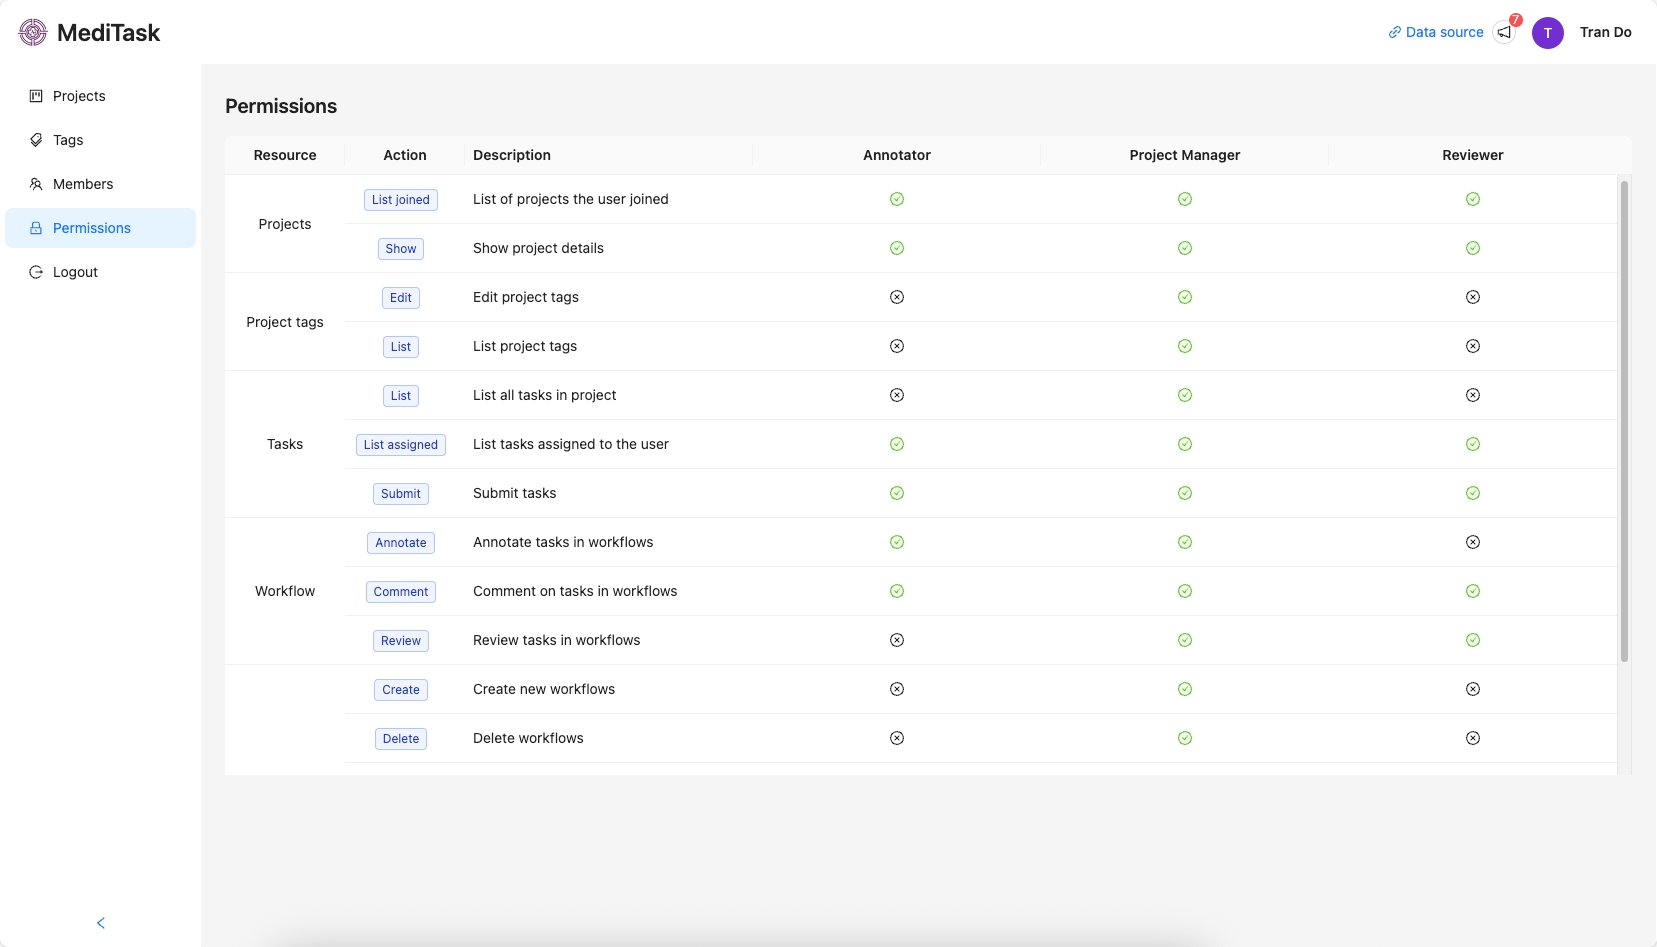
\includegraphics[width=1\textwidth]{content//resources//features//permissions.png}
    \caption{Granular Permissions Configuration Interface}
    \label{fig:permissions-config}
\end{figure}

\subsection{Workflow Management}
At the heart of the platform lies a powerful and adaptable workflow engine that facilitates the construction and execution of complex data processing pipelines.

\subsubsection{Dynamic Workflow Graphs}
Workflows are visually represented and defined as directed graphs, comprising interconnected stages (nodes) and connections (edges). This graph structure is customizable per project, allowing for bespoke data processing flows. Figure~\ref{fig:workflow-editor-simple} illustrates the intuitive drag-and-drop interface for designing workflows, while Figure~\ref{fig:workflow-editor-advanced} demonstrates a more complex workflow incorporating routing and consensus stages.

\begin{figure}[h!]
    \centering
    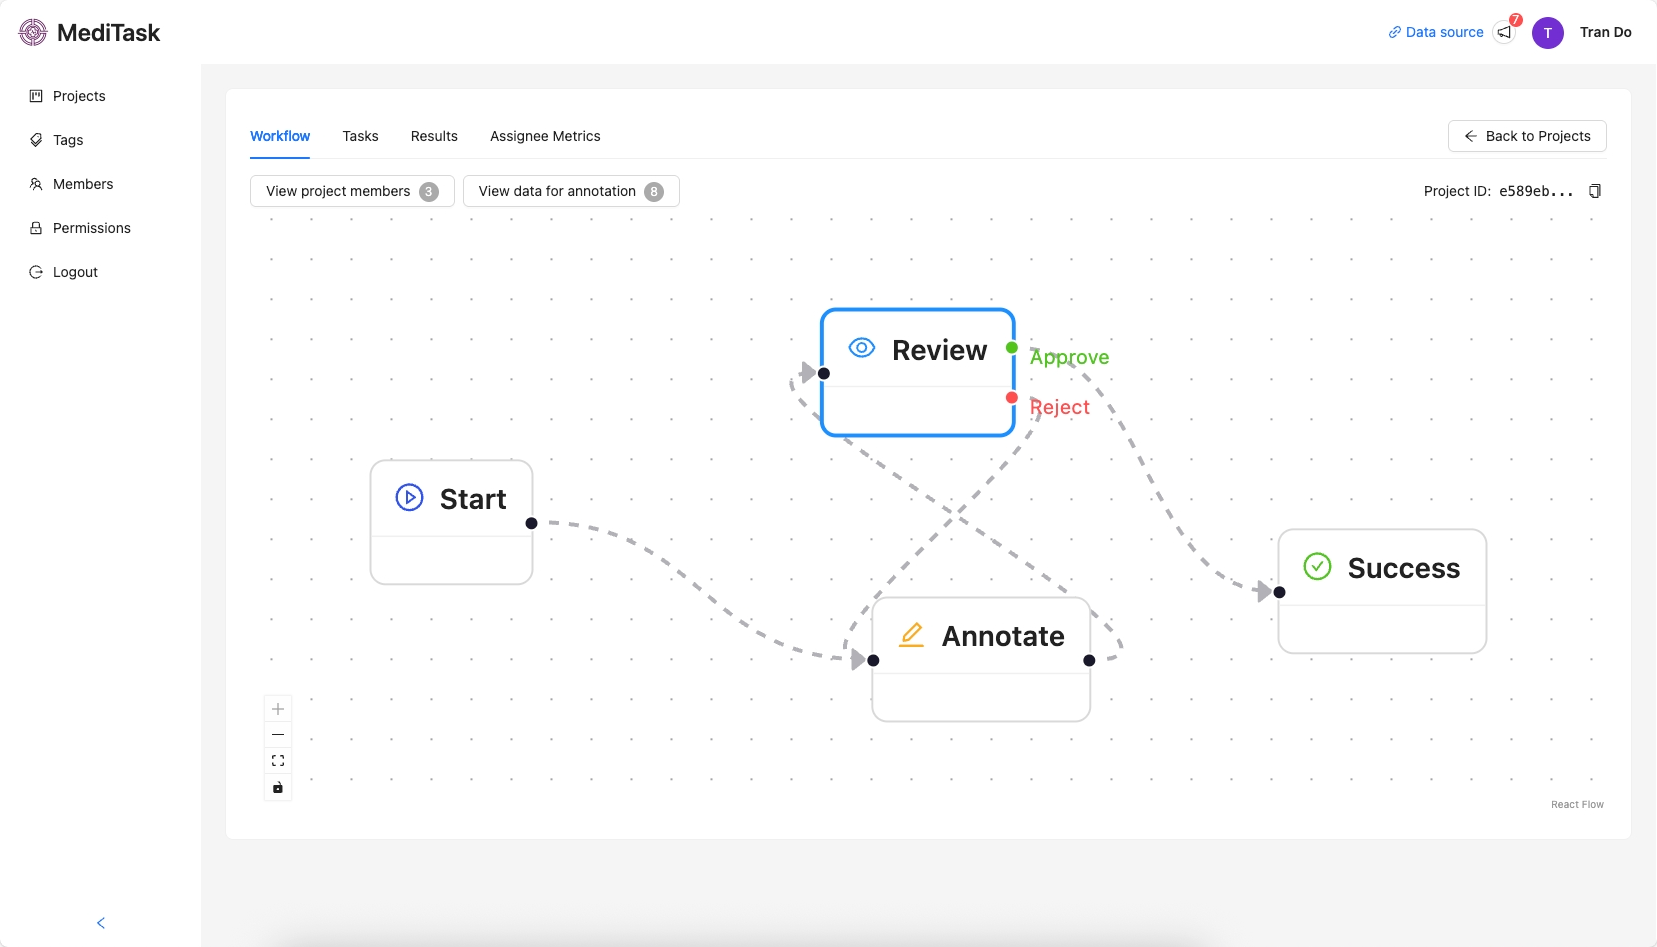
\includegraphics[width=1\textwidth]{content/resources/features/simple workflow.png}
    \caption{Workflow Design Interface}
    \label{fig:workflow-editor-simple}
\end{figure}

\begin{figure}[h!]
    \centering
    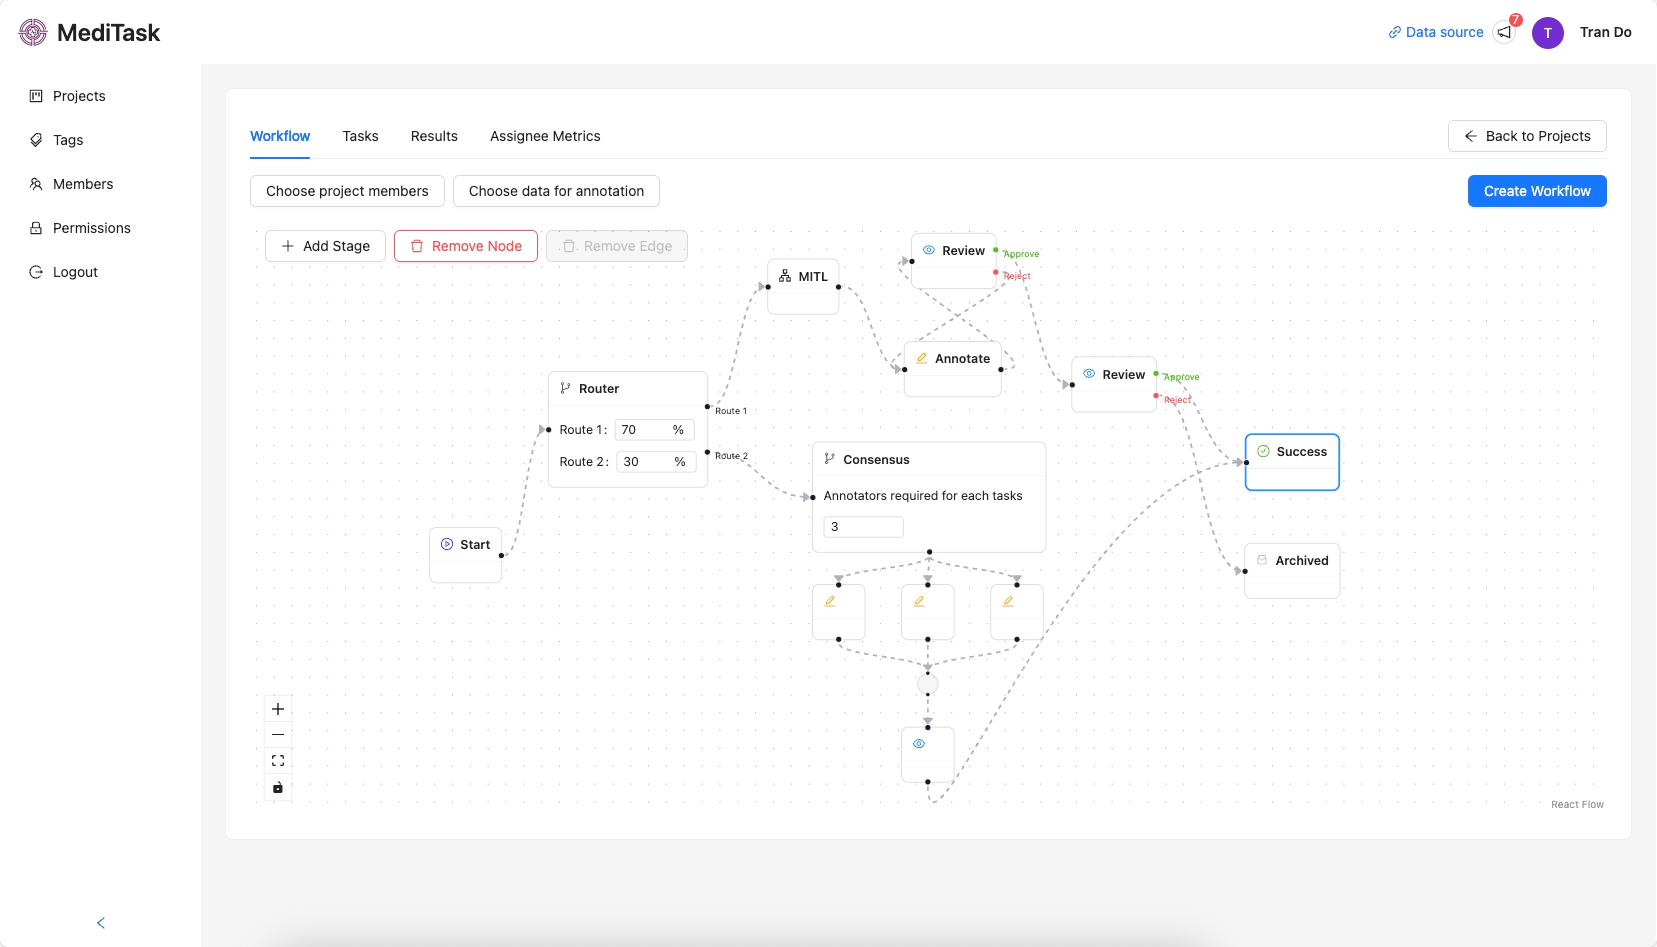
\includegraphics[width=1\textwidth]{content/resources/features/complex workflow.png}
    \caption{Advanced Workflow with Router and Consensus Stages}
    \label{fig:workflow-editor-advanced}
\end{figure}

\subsubsection{Customizable Stages and Conditional Logic}
Each workflow stage possesses a distinct type (e.g., \texttt{ANNOTATE}, \texttt{REVIEW}, \texttt{CONSENSUS}) and can host unique custom configurations. The system supports advanced conditional branching, enabling distinct success and failure paths for tasks at each stage, ensuring resilient workflow progression. As shown in Figure~\ref{fig:workflow-select-members}, users can easily select project members and their roles, which can then be assigned to workflow stages.

\begin{figure}[h!]
    \centering
    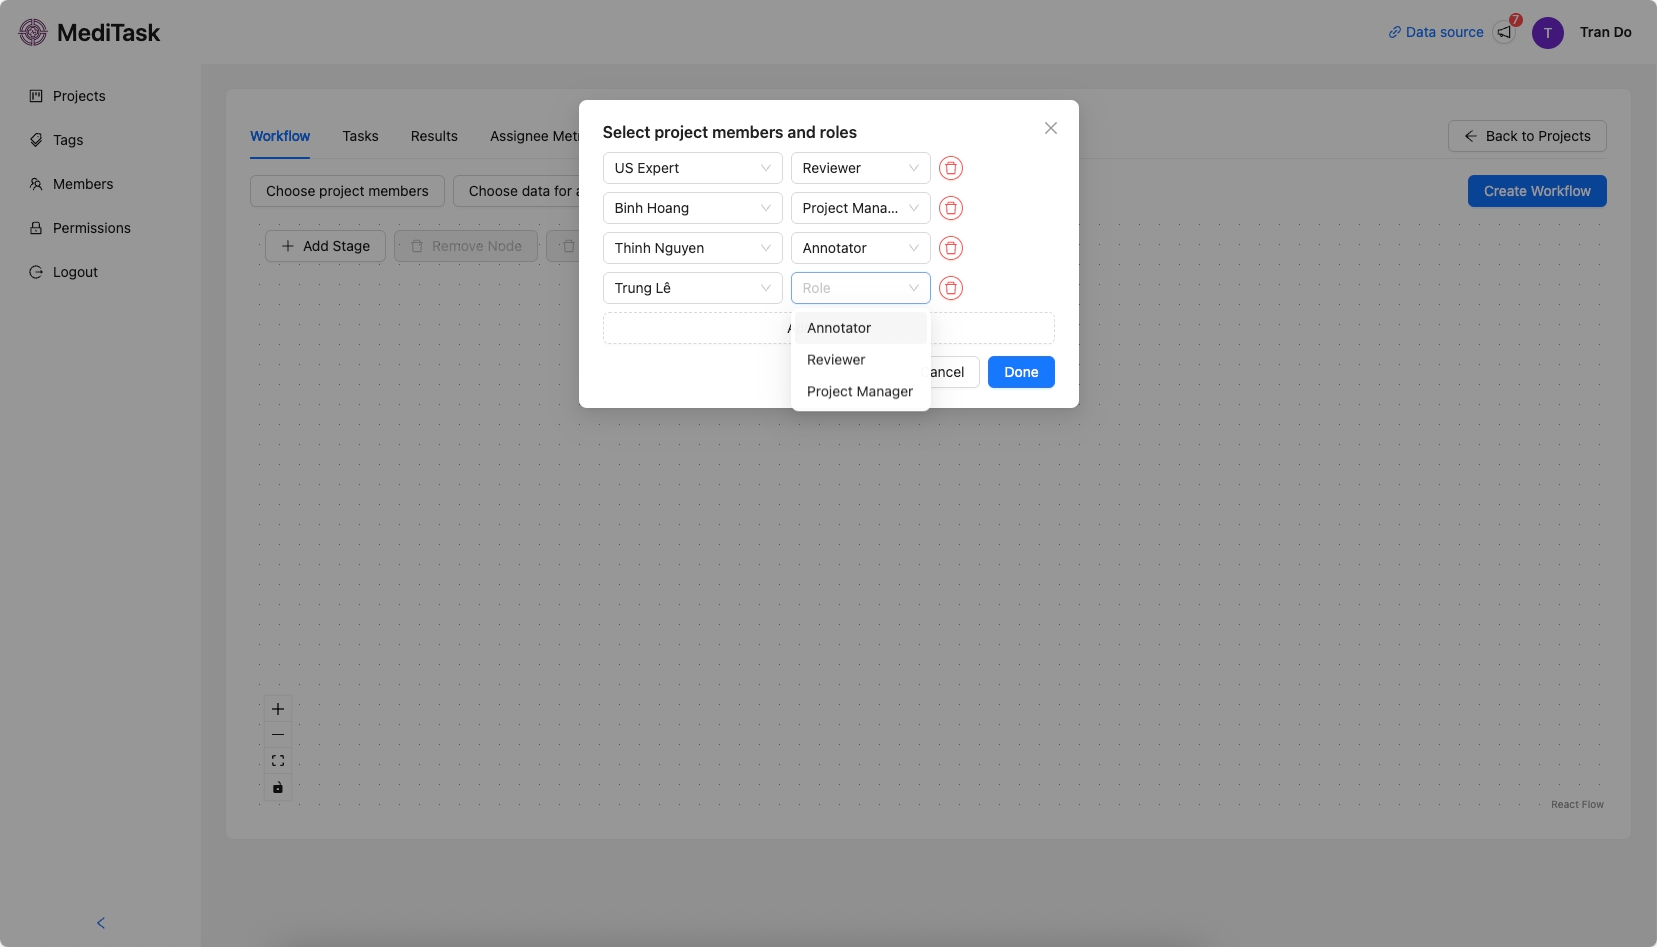
\includegraphics[width=0.6\textwidth]{content/resources/features/choose members.png}
    \caption{Selecting Project Members for Workflow Assignment}
    \label{fig:workflow-select-members}
\end{figure}

\subsubsection{Automated Assignee Selection}
The platform can automatically determine the subsequent assignee for a task based on functions linked to each workflow stage. This capability underpins complex routing logic, optimizing task distribution and flow. Figure~\ref{fig:workflow-select-data} demonstrates the process of selecting specific data instances to be included in a workflow, ensuring only relevant data undergoes the defined process.

\begin{figure}[h!]
    \centering
    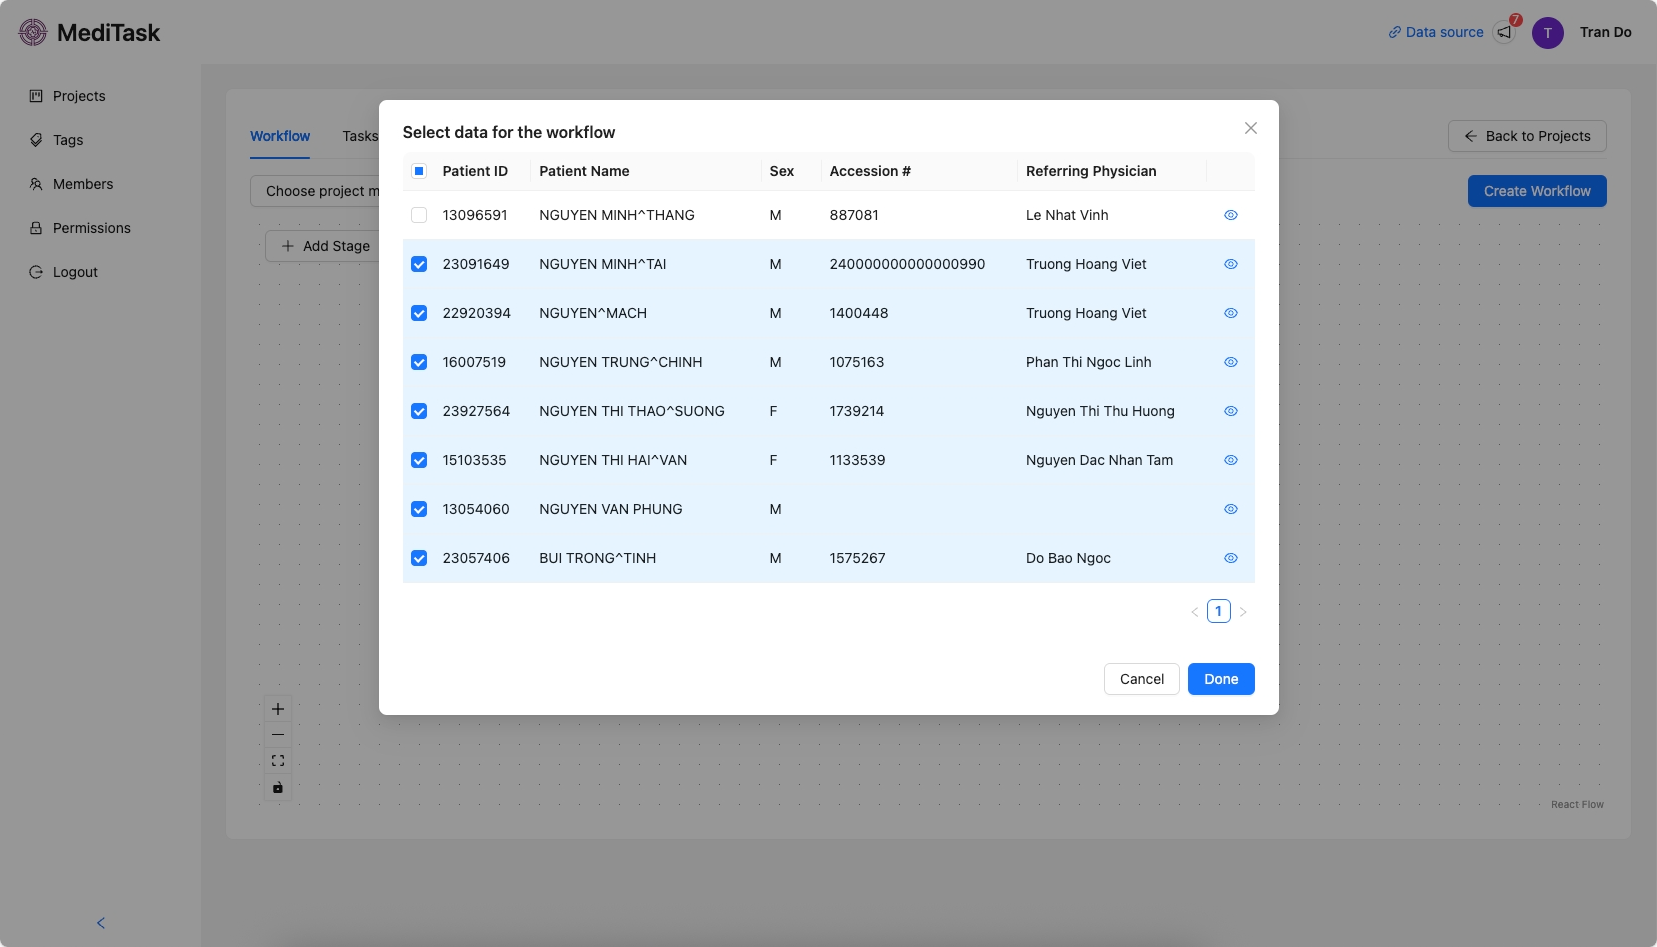
\includegraphics[width=0.6\textwidth]{content/resources/features/choose dataset.png}
    \caption{Selecting Data Instances for Workflow Processing}
    \label{fig:workflow-select-data}
\end{figure}

\subsection{Project \& Task Management}
Comprehensive tools are provided for the organization and management of projects and their constituent tasks.

\subsubsection{Centralized Project Hub}
Projects serve as the primary organizational unit, encapsulating datasets, tasks, and member assignments. Each project is defined by a name, description, and an associated set of members, providing a consolidated view for all related activities. Figure~\ref{fig:project-list} illustrates the centralized project hub, allowing users to overview and manage their ongoing annotation efforts. Projects can also be categorized using a flexible, color-coded tagging system, enhancing visual identification and search capabilities, as seen in Figure~\ref{fig:tags-list}.

\begin{figure}[h!]
    \centering
    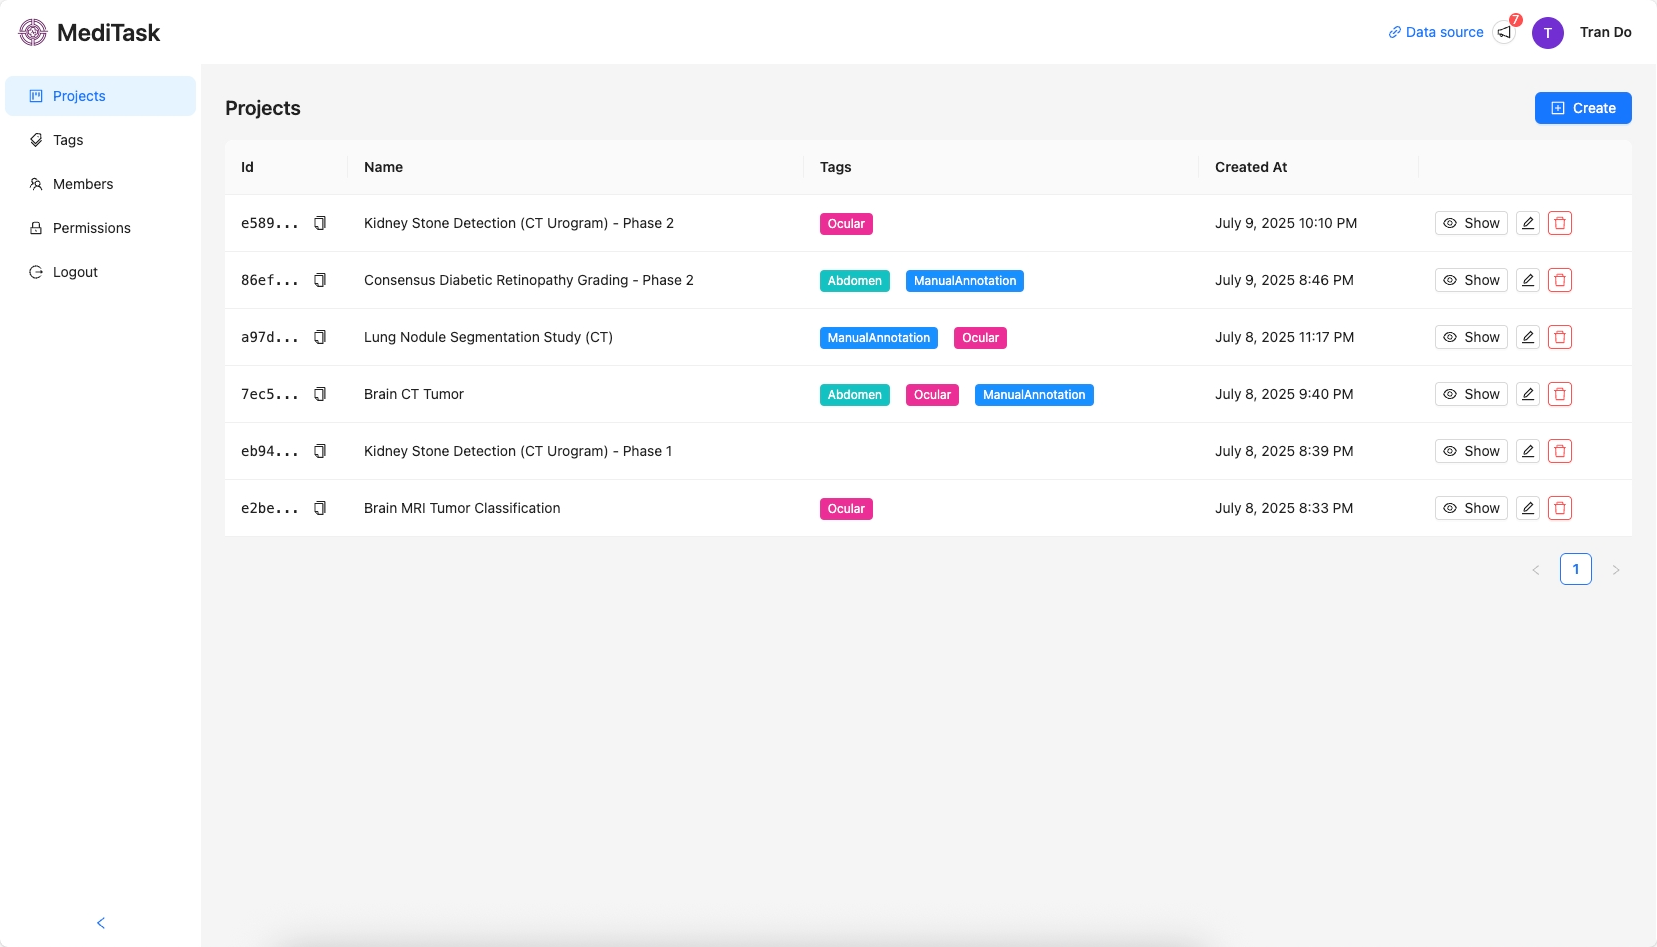
\includegraphics[width=1\textwidth]{content//resources//features//projects.png}
    \caption{Layout of Project Management Page}
    \label{fig:project-list}
\end{figure}

\begin{figure}[h!]
    \centering
    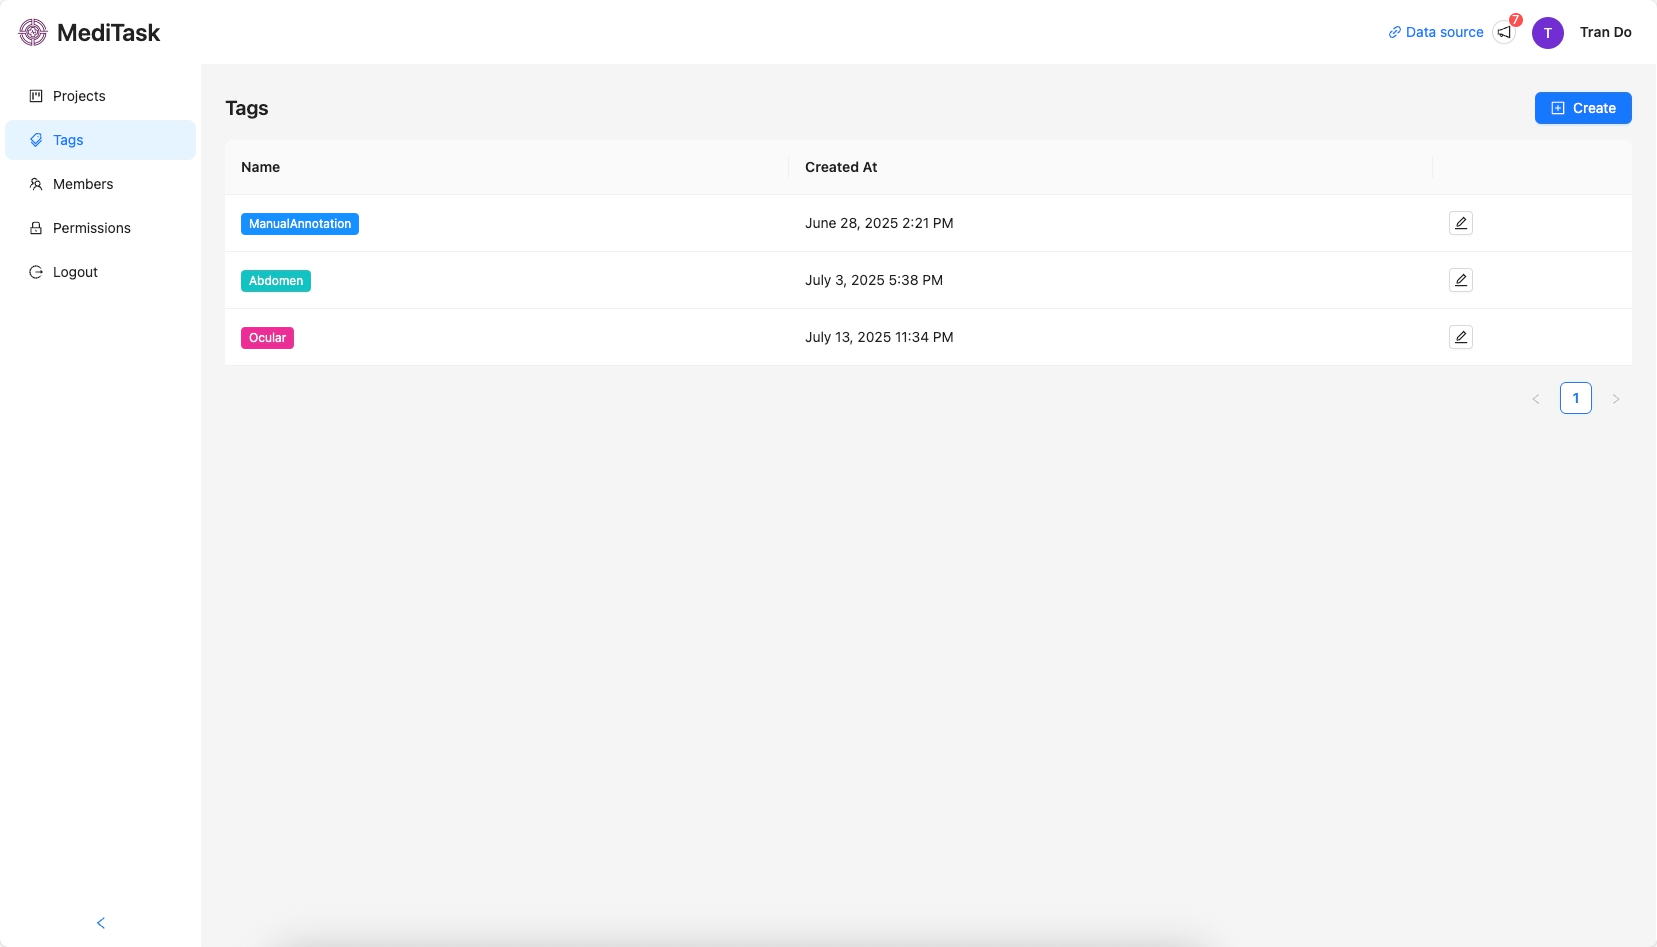
\includegraphics[width=1\textwidth]{content//resources//features//tags.png}
    \caption{Project Tag Management Interface}
    \label{fig:tags-list}
\end{figure}

\subsubsection{Task Lifecycle Management}
Tasks represent discrete units of work tied to specific data items. They transition through various statuses (e.g., \texttt{PENDING}, \texttt{COMPLETED}) as they advance through the defined workflow, ensuring clear visibility of progress. Figure~\ref{fig:tags-list} and Figure~\ref{fig:tasks-tab-1} showcase different views of the task list within a project, providing comprehensive oversight of task status, assignment, and progress.

\begin{figure}[h!]
    \centering
    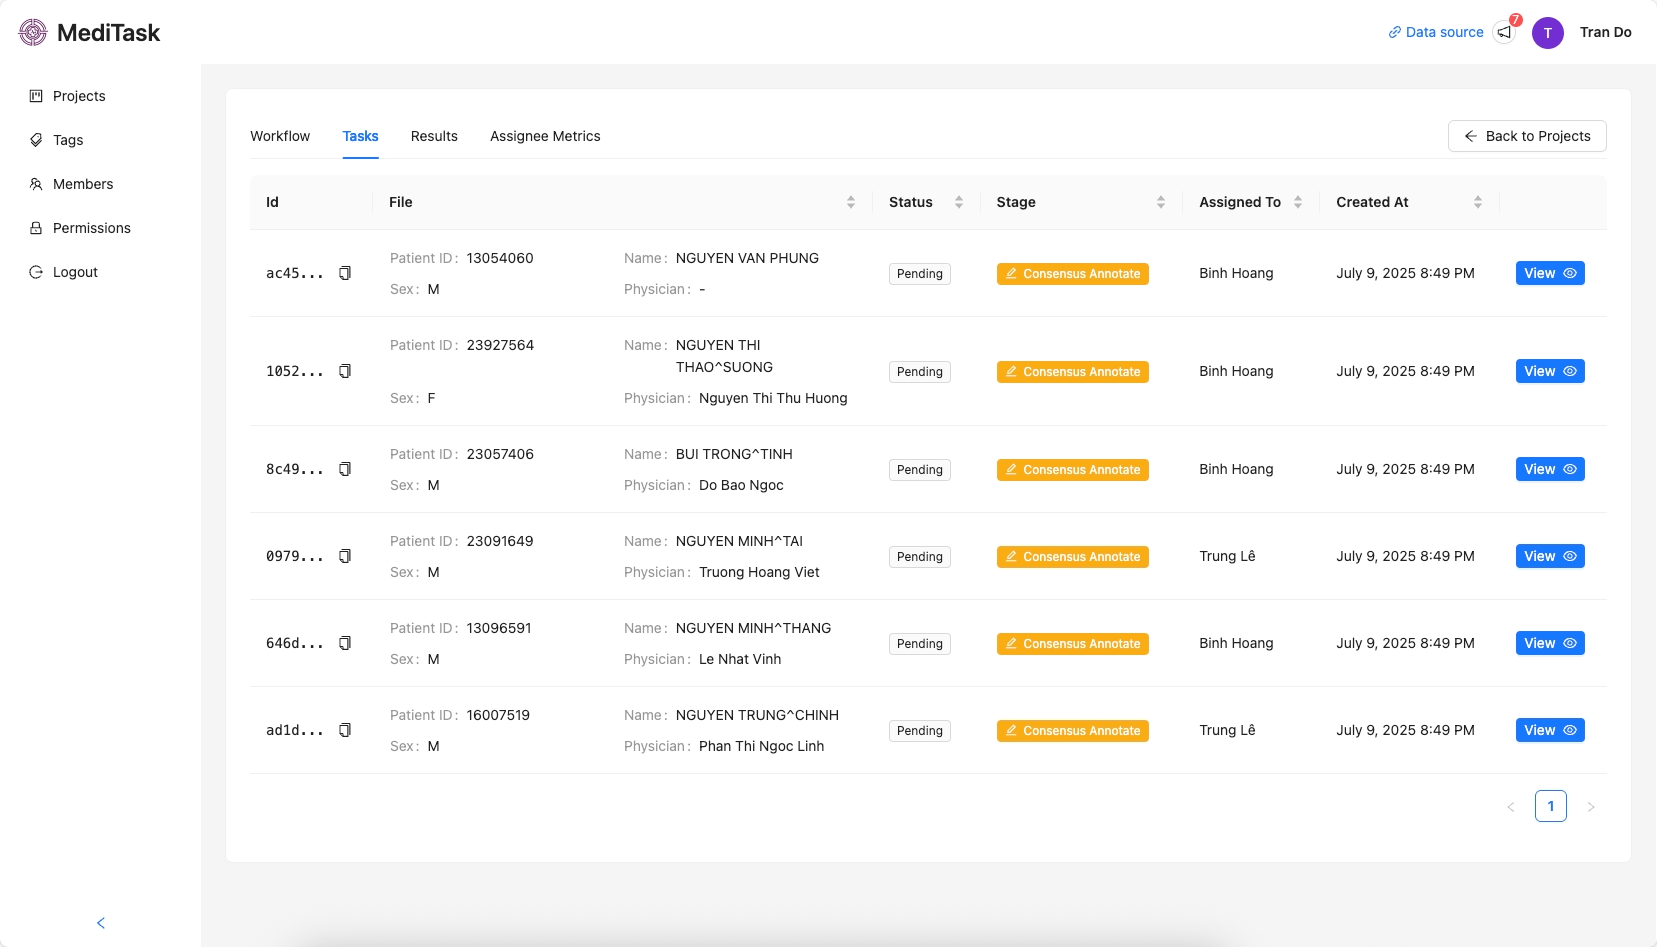
\includegraphics[width=1\textwidth]{content/resources/features/tasks.png}
    \caption{Task List View within a Project}
    \label{fig:tasks-tab-1}
\end{figure}

\subsubsection{Detailed Task Assignments}
Task progression through a workflow is managed via assignments. Each assignment links a task to a specific user at a particular workflow stage, meticulously tracking its status, start time, and completion time, creating an auditable trail.

\subsection{Member Management}
The platform facilitates the effective management of users and their roles within projects.

\subsubsection{User and Project-Level Role Management}
Administrators can create, list, and modify user accounts within the system. Critically, roles are assigned on a per-project basis, allowing for granular control over user permissions and responsibilities tailored to each project's needs. While a dedicated member list view is not shown, the `Permissions` interface (Figure~\ref{fig:permissions-config}) implicitly demonstrates the role-based access control for different user types.

\subsection{Annotation \& Collaboration}
The platform is meticulously designed to foster efficient and accurate data annotation through a robust collaborative environment.

\subsubsection{Integrated Annotation Tools}
The system seamlessly integrates with industry-standard tools such as OHIF Viewer, MONAI, and Orthanc. This integration supports advanced medical imaging annotation workflows and enables AI-assisted labeling functionalities. Figure~\ref{fig:annotation-viewer} provides a view of the integrated medical imaging annotation environment, while Figure~\ref{fig:orthanc-integration} shows the external Orthanc integration for data source management.

\begin{figure}[h!]
    \centering
    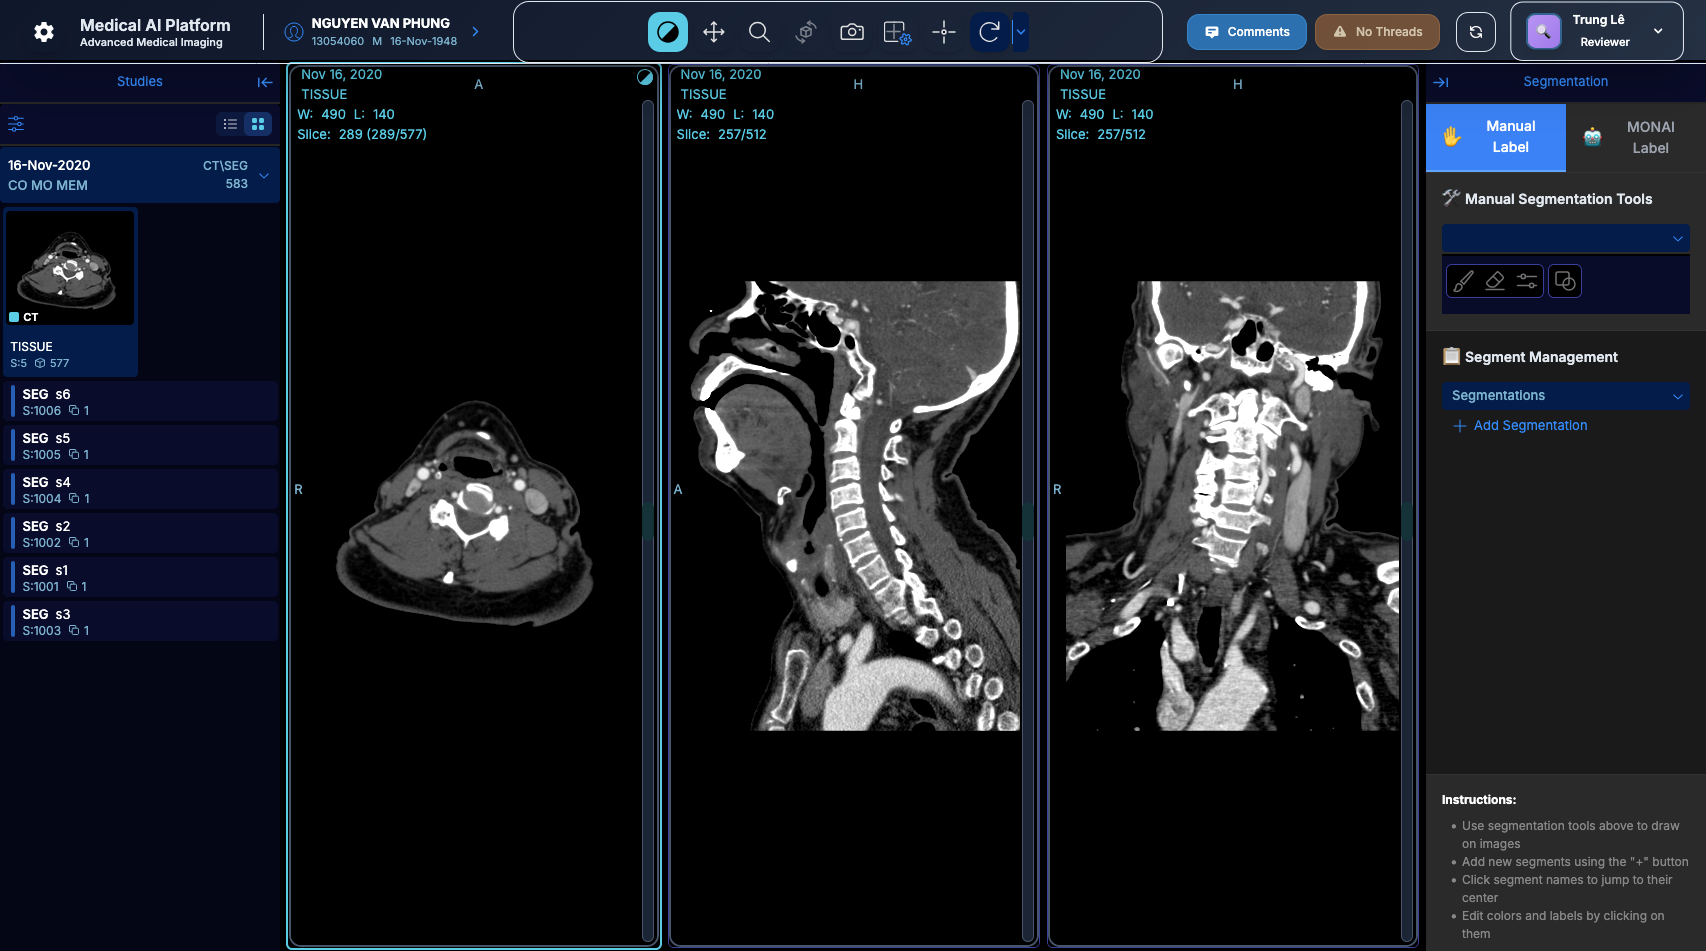
\includegraphics[width=1\textwidth]{content/resources/features/ohif.png}
    \caption{Integrated Medical Imaging Annotation Viewer}
    \label{fig:annotation-viewer}
\end{figure}

\subsubsection{Annotation Commenting and Segmentation Data}
Users can leave rich, structured comments on task assignments, facilitating detailed discussions and feedback loops. Figure~\ref{fig:annotation-comments} illustrates the task assessment hub, which includes a dedicated section for comments and collaboration. Tasks are also capable of storing lists of segmentation IDs, which are crucial for image-based annotation tasks involving precise object boundaries.

\begin{figure}[h!]
    \centering
    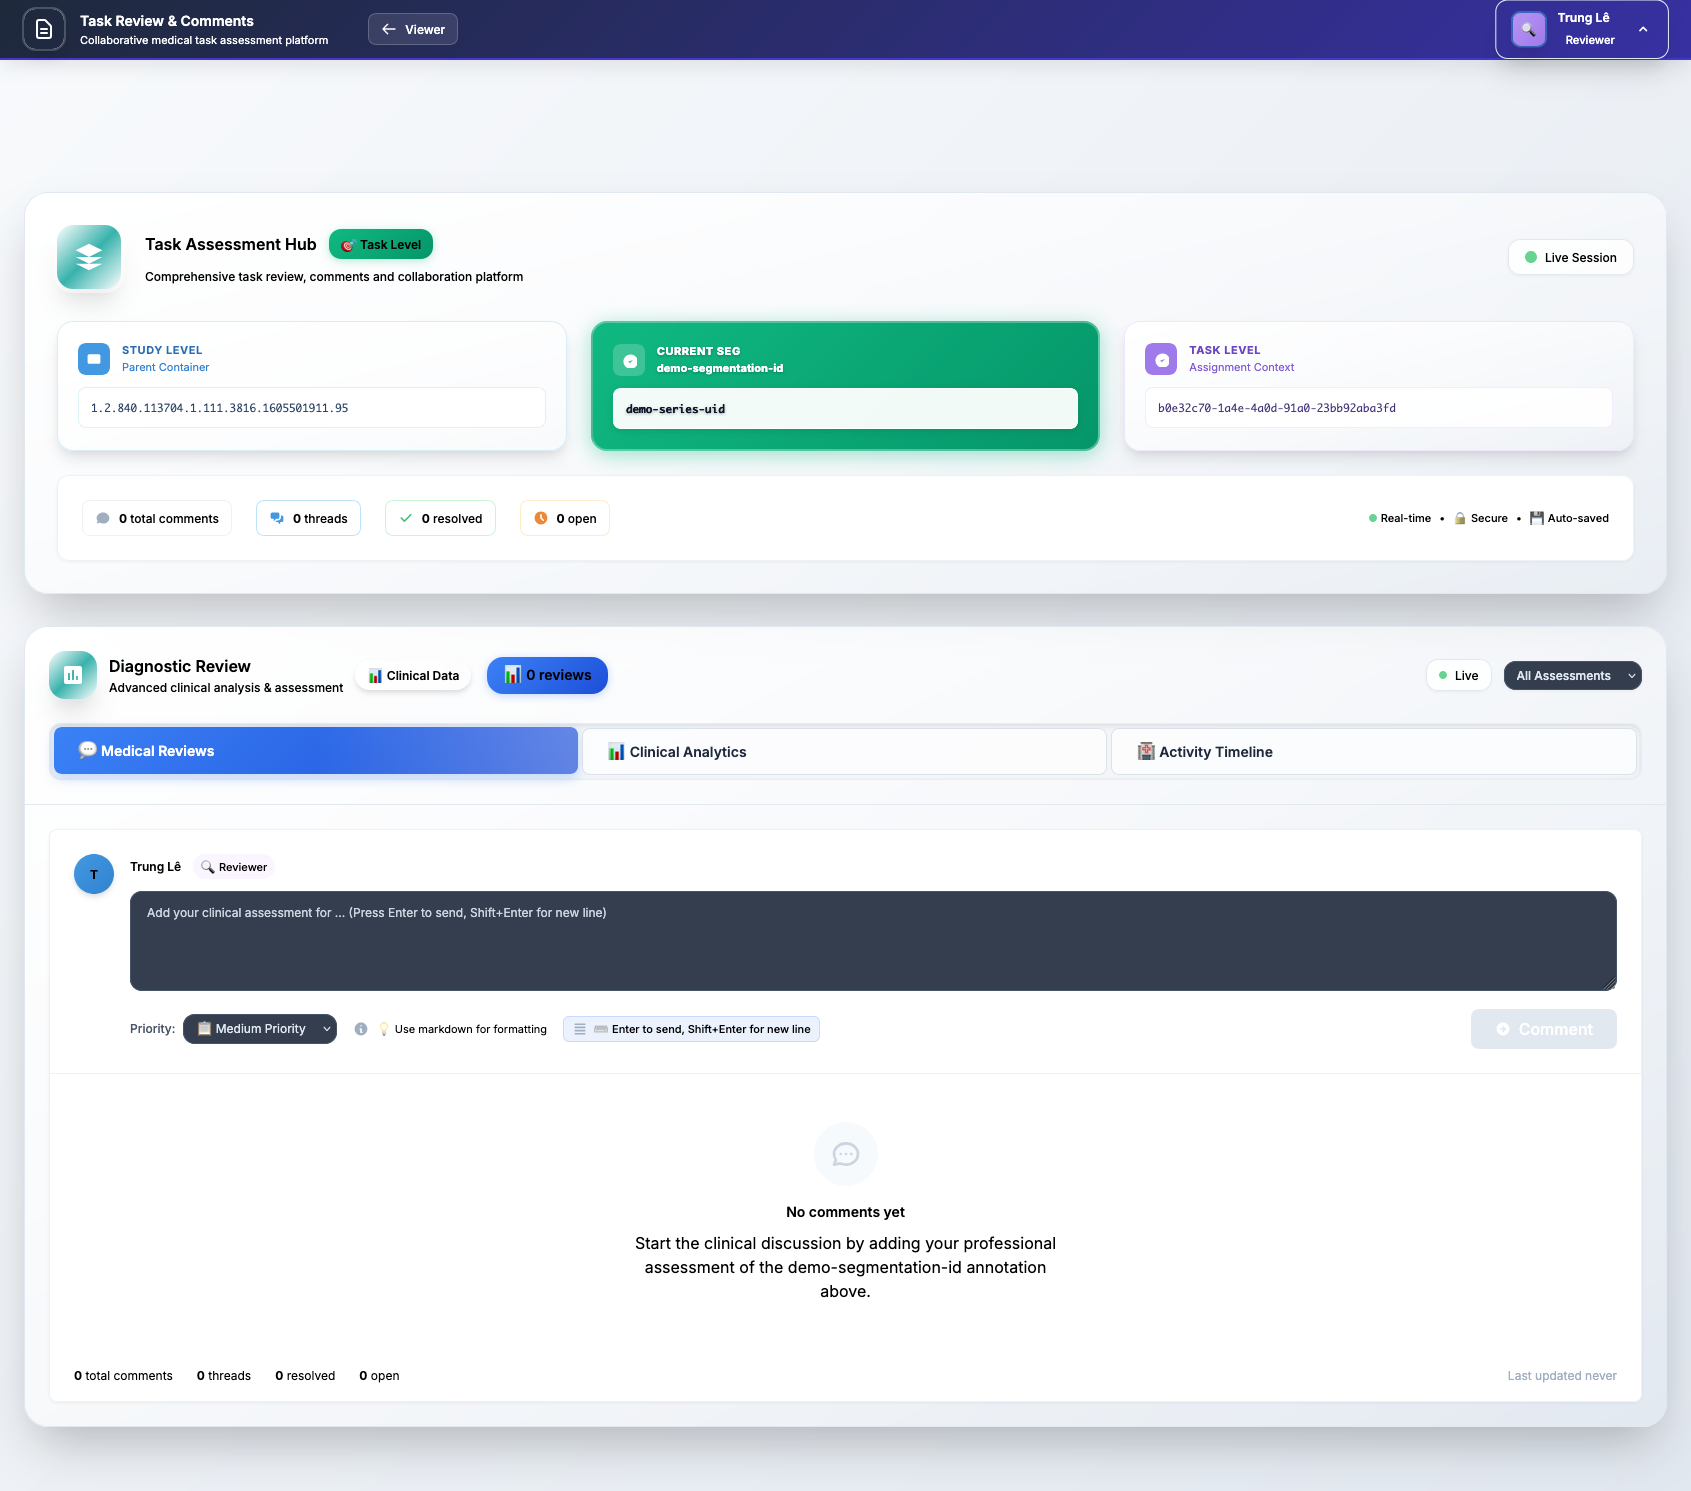
\includegraphics[width=1\textwidth]{content/resources/features/ohif comment.png}
    \caption{Task Assessment Hub with Annotation Commenting}
    \label{fig:annotation-comments}
\end{figure}

\subsubsection{Data Source Integration}
The system can connect to and ingest data items from external sources, including specialized medical imaging archives like Orthanc, streamlining the data acquisition process for annotation.

\begin{figure}[h!]
    \centering
    \includegraphics[width=1\textwidth]{content//resources//features//orthanc.png}
    \caption{Orthanc Data Source Integration Interface}
    \label{fig:orthanc-integration}
\end{figure}

\subsection{Backend Automation: Virtual Users and Cron-Based Workflow Orchestration}
A cornerstone of the platform's backend architecture is its capacity for automated workflow progression, reducing the need for direct human intervention in repetitive or system-driven tasks. This is achieved through a synergy of "virtual users" and scheduled cron jobs, forming an intelligent, SQL-based orchestration layer.

\subsubsection{The Concept of Virtual Users}
To manage automated, non-human operations, the system employs "virtual users." These are specialized user accounts within the `\_users` table, distinguished by an `is\_system` boolean field set to `true`. They act as system-level actors for specific automated functions, such as:
\begin{itemize}
    \item \textbf{START}: Initiates new tasks in a workflow.
    \item \textbf{ROUTER}: Manages conditional logic, directing tasks based on predefined rules embedded in workflow stage configurations.
    \item \textbf{CONSENSUS}: Orchestrates the aggregation and comparison of multiple annotations to determine agreement, critical for quality control.
\end{itemize}
When a task enters a stage requiring automated processing, it is assigned to one of these virtual users within the `\_task\_assignments` table, awaiting system action.

\subsubsection{Cron Jobs: The Automation Trigger}
Unlike human-initiated tasks, tasks assigned to virtual users are processed by scheduled cron jobs. These are PostgreSQL functions configured to execute at regular intervals (e.g., every minute), establishing a robust polling mechanism. Key cron jobs for workflow automation include `workflow\_start`, `workflow\_route`, `workflow\_consensus`, and `workflow\_consensus\_holding`.

\subsubsection{The Automated Orchestration Flow}
The automated workflow progresses through a clear, stateful sequence recorded within the database:
\begin{enumerate}
    \item \textbf{Assignment to Virtual User}: A task transitions to an automated stage (e.g., a `ROUTER` stage), triggering the creation of a new `\_task\_assignments` record that links the task to the stage and the relevant virtual user.
    \item \textbf{Scheduled Execution}: A periodically running cron job (e.g., `workflow\_route()`) is invoked.
    \item \textbf{Task Processing}: The executing function queries `\_task\_assignments` for all 'PENDING' tasks assigned to its corresponding virtual user.
    \item \textbf{Logic Execution}: For each pending task, the function executes specialized logic. For a `ROUTER` stage, this involves interpreting the `custom\_config` JSONB field from the `\_workflow\_stages` entry to determine the next path.
    \item \textbf{Workflow Progression}: Upon logic execution, the function advances the task to the next stage by:
    \begin{itemize}
        \item Updating the current assignment's status to 'COMPLETED'.
        \item Determining the subsequent stage ID using `on\_success\_stage\_id` or `on\_failure\_stage\_id`.
        \item Creating a new `\_task\_assignments` record for the next stage, assigning it to the appropriate human or virtual user. The `previous\_task\_assignment\_id` is linked to the completed assignment, ensuring an immutable and auditable event chain.
    \end{itemize}
\end{enumerate}
This cron-based approach establishes a powerful, asynchronous, and fully automated backend engine, driving the workflow forward in a serverless architecture.

\begin{figure}[h!]
    \centering
    % \includegraphics[width=0.8\textwidth]{path/to/your/workflow\_automation\_flow.png} % No specific image provided for this abstract concept.
    \caption{Conceptual Workflow Automation Flow}
    \label{fig:automation-flow}
\end{figure}

\subsection{Notifications}
A robust, built-in notification system ensures users are continuously informed about critical events and workflow updates.

\subsubsection{Event-Driven Notifications with Custom Payloads}
Users receive timely notifications for key events, such as new task assignments or actions requiring their attention. Each notification carries a custom payload, providing contextual data directly to the user, enhancing actionable information. Figure~\ref{fig:notifications} shows the notification panel, providing a chronological list of updates.

\begin{figure}[h!]
    \centering
    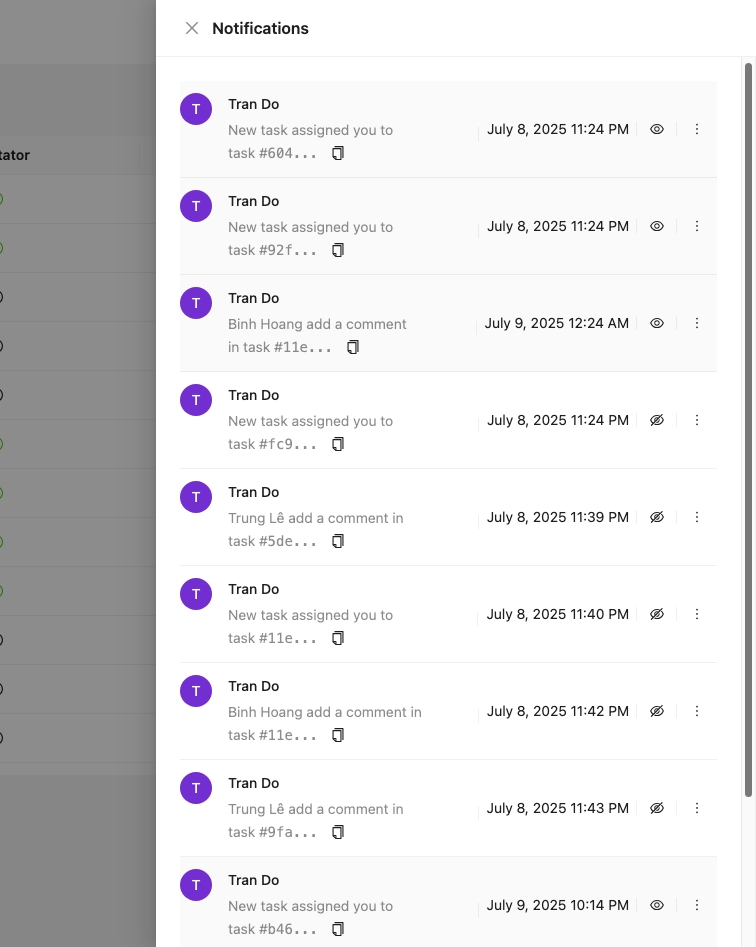
\includegraphics[width=0.6\textwidth]{content//resources//features//notifications.png}
    \caption{User Notification Panel}
    \label{fig:notifications}
\end{figure}

\subsubsection{View Tracking}
The system tracks notification viewing status, ensuring users do not miss critical updates and facilitating effective communication within the platform.

\subsection{System Integrations}
The platform is designed with extensibility in mind, allowing for seamless integration with external systems and machine learning models.

\subsubsection{Machine Learning Model Integration}
The system can connect to external ML models by storing their API endpoints. This capability enables advanced features such as model-assisted labeling (MITL), enhancing annotation efficiency and accuracy.

\section{Demo Plan}
\subsection{Metadata Auto Extraction with Q\&A Pairs Generation}
\begin{itemize}
    \item \textbf{Step 1: Input}
    \begin{itemize}
        \item \textbf{Action:} Input a full description of SeLab into the input box, along with the exact position.
        \item \textbf{Expected Result:} No immediate output is generated.
    \end{itemize}
    
    \item \textbf{Step 2: Q\&A Pair Generation}
    \begin{itemize}
        \item \textbf{Action:} Click the \emph{Generate} button.
        \item \textbf{Expected Result:} The app displays a generating process (from 0--100\%). Once complete, a new screen presents the generated Q\&A pairs.
    \end{itemize}
    
    \item \textbf{Step 3: Regeneration}
    \begin{itemize}
        \item \textbf{Action:} Click the \emph{Regenerate} button.
        \item \textbf{Expected Result:} The app displays the generating process again. A new screen shows a slightly different set of Q\&A pairs when finished.
    \end{itemize}
    
    \item \textbf{Step 4: Submission}
    \begin{itemize}
        \item \textbf{Action:} Click the \emph{Submit} button.
        \item \textbf{Expected Result:} The app shows the submission process (from 0--100\%), and upon completion, notifies the user that the metadata has been successfully updated to the remote database.
    \end{itemize}
\end{itemize}

\subsection{Indoor Space -- Floor 7th and 8th}
\begin{itemize}
    \item \textbf{Step 1: Initiate AR Session}
    \begin{itemize}
        \item \textbf{Action:} Scan the QR code located on the 8th floor.
        \item \textbf{Expected Result:} The system automatically launches the AR camera session.
    \end{itemize}
    
    \item \textbf{Step 2: Location Tracking}
    \begin{itemize}
        \item \textbf{Action:} Walk between the 7th and 8th floors and move the camera into unknown locations.
        \item \textbf{Expected Result:} The system updates and notifies the current location as the user moves between floors and warns when entering undetected environments.
    \end{itemize}
    
    \item \textbf{Step 3: Activate AI Assistance}
    \begin{itemize}
        \item \textbf{Action:} Greet the AI assistant.
        \item \textbf{Expected Result:} The AI assistant responds with guidance on how to query for a destination.
    \end{itemize}
    
    \item \textbf{Step 4: Query to I77}
    \begin{itemize}
        \item \textbf{Action:} Query “Find the path to the I77 room.”
        \item \textbf{Expected Result:} The system displays a clear navigation path leading to the I77 room.
    \end{itemize}
    
    \item \textbf{Step 5: Follow the Navigation Path}
    \begin{itemize}
        \item \textbf{Action:} Walk following the on-screen arrows.
        \item \textbf{Expected Result:} Upon arrival at the I77 room, the system notifies the user that they have reached the destination.
    \end{itemize}
    
    \item \textbf{Step 6: Query for the Research Room}
    \begin{itemize}
        \item \textbf{Action:} Query “How do I get to the research room?”
        \item \textbf{Expected Result:} The system responds with an ambiguity alert, indicating that multiple rooms could match the query (e.g., I87 and I77) and requests more information.
    \end{itemize}
    
    \item \textbf{Step 7: Clarify Destination for Software Engineering}
    \begin{itemize}
        \item \textbf{Action:} Query more specifically “Show path to the room for researching about Software Engineering.”
        \item \textbf{Expected Result:} The system displays the navigation path to the I87 room.
    \end{itemize}
    
    \item \textbf{Step 8: Query for a Room on Floor 8}
    \begin{itemize}
        \item \textbf{Action:} Query “Find the path to the room on floor 8.”
        \item \textbf{Expected Result:} The system again flags the query as ambiguous, indicating that multiple rooms could match the query (e.g., I87 and the restroom on floor 8) and requests more information..
    \end{itemize}
    
    \item \textbf{Step 9: Specify Research Room on Floor 8}
    \begin{itemize}
        \item \textbf{Action:} Combine the vague details by querying “Show me the path to the room for research on floor 8.”
        \item \textbf{Expected Result:} The system correctly displays the navigation path to the I87 room.
    \end{itemize}
\end{itemize}

\subsection{Semi-outdoor Space -- Front Campus of HCMUS}
\begin{itemize}
    \item \textbf{Step 1: Initiate AR Session}
    \begin{itemize}
        \item \textbf{Action:} Scan the QR code at the front gate.
        \item \textbf{Expected Result:} The AR camera session is activated, launching the AR interface in the semi-outdoor environment.
    \end{itemize}
    
    \item \textbf{Step 2: Verify AR Tracking}
    \begin{itemize}
        \item \textbf{Action:} Pan and move the camera around the area.
        \item \textbf{Expected Result:} The system confirms continuous tracking and reliable environment detection.
    \end{itemize}
    
    \item \textbf{Step 3: Query for the Ground Elevator}
    \begin{itemize}
        \item \textbf{Action:} Query “Find the path to the ground elevator of building I.”
        \item \textbf{Expected Result:} The system displays a clear navigation path leading to the ground elevator.
    \end{itemize}
    
    \item \textbf{Step 4: Follow the Navigation Path}
    \begin{itemize}
        \item \textbf{Action:} Walk following the on-screen arrows.
        \item \textbf{Expected Result:} The user arrives at the ground elevator of building I.
    \end{itemize}
    
    \item \textbf{Step 5: Query for the Parking Lot}
    \begin{itemize}
        \item \textbf{Action:} Query “Find the path to the parking lot.”
        \item \textbf{Expected Result:} The system flags the query as ambiguous due to multiple parking lots, requesting additional clarification.
    \end{itemize}
    
    \item \textbf{Step 6: Specify the Underground Parking Lot}
    \begin{itemize}
        \item \textbf{Action:} Query “Show me the path to the underground parking lot.”
        \item \textbf{Expected Result:} The system displays a clear navigation route to the underground parking lot.
    \end{itemize}
\end{itemize}
